
\section{$V_{cs}$ From $B(W\to l \nu)$ }
\label{sec:relatedWorks:vcs}

\subsection{Overview of $V_{cs}$ Measurements}

The CKM matrix originates from the Yukawa couplings in the SM Higgs sector. It represents the mixing of the quarks' mass eigenstates when forming the flavor eigenstates. So when physical quarks in their mass eigenstates participate in the weak interaction, they are projected to the flavor eigenstates first using the corresponding element in the CKM matrix. More details about the CKM in the standard model are discussed in Section~\ref{sec:relatedWorks:qft:gws}. 

\begin{table}[ht]
    \centering
    \setlength{\tabcolsep}{1.5em}
    \renewcommand{\arraystretch}{1.5}
    \begin{tabular}{c|c|c }
        \hline
         $|V_{ud}|=0.97370 \pm 0.00014 $         & $|V_{us}|=0.2245 \pm 0.0008$       &  $|V_{ub}|=0.00382 \pm 0.00024$         \\ \hline
       $|V_{cd}|=0.221 \pm 0.004 $                    & $|V_{cs}|=0.987 \pm 0.011$       &  $|V_{cb}|=0.00410 \pm 0.0014$                    \\ \hline
       $|V_{td}|=0.0080 \pm 0.0003 $               & $|V_{ts}|=0.0388 \pm 0.0011$       &  $|V_{tb}|=1.013 \pm 0.030$                    \\
        \hline
    \end{tabular}
    \caption{The current experimental world average of the 9 elements in the CKM matrix in the PDG \cite{pdg2020}.  }
    \label{tab:relatedWorks:vcs:ckm}
\end{table}


The current experimental measurement of the 9 elements in the CKM matrix \cite{pdg2020} is shown in Table~\ref{tab:relatedWorks:vcs:ckm}. Among the 6 elements in the first two rows, the $|V_{cs}|$ is measured with the least precision. The average of $|V_{cs}|$ measurements is shown in Figure~\ref{fig:relatedWorks:vcs:measurements}. Currently, there are two direct approaches to measure $|V_{cs}|$, using the D meson decay in the charm factories and using the on-shell $W\to c s$  with jet tagging in the collider experiments.

The best direct determination of $|V_{cs}|$ is from the semileptonic decay of $D$ and the leptonic decay of $D_s$ produced in the charm factory. For the results from the leptonic decay of $D_s$ meson, the branching fraction of $D_s^+ \to \mu^+ \nu$ and $D_s^+ \to \tau^+ \nu$ are both measured in the Belle \cite{Zupanc:2013byn}, CLEO \cite{Alexander:2009ux,Onyisi:2009th,Naik:2009tk}, BaBar \cite{delAmoSanchez:2010jg} and BESIII \cite{Ablikim:2016duz, Ablikim:2018jun}. Using the experimental value of mass and lifetime of $D_s$, as well as the lattice QCD calculation of the form factor $f_{D_s}$, $|V_{cs}|$ can be determined from the $D_s$ leptonic decay and yields a world average of $|V_{cs}|=0.992\pm 0.012$ \cite{Amhis:2019ckw}, where the dominating uncertainty is from the experimental error. For the results from the semileptonic decay of $D$ meson, the branching fraction of $D\to K l\nu$ is measured by CLEO-c \cite{Besson:2009uv}, Belle \cite{Widhalm:2006wz}, BaBar \cite{Aubert:2007wg} and BESIII \cite{Ablikim:2015ixa, Ablikim:2018evp}, which gives an average of $|V_{cs}|$ of $|V_{cs}|=0.939\pm 0.038$ \cite{Amhis:2019ckw} in the D meson decay. The dominant uncertainty is form the theoretical calculations of the D meson form factor with latice QCD. Combining the result from the $D$ and $D_s$ decay, the charm factories measures $|V_{cs}|=0.987\pm 0.011$ \cite{Amhis:2019ckw}.

The second direct measurement of $|V_{cs}|$ is from the on-shell $W\to c s$ decays in the collider experiments. This approach relies on jet tagging to identifies the jets originating from the c and s quarks, which is relatively difficult, especially in the hadron collider with a more complex hadron environment. Therefore, this approach is less explored compared with the $D/D_s$ approach. So far, the only published result in the $W\to c s$  approach is from the DELPHI in the LEP, which reports $|V_{cs}|=0.94 ^{+0.32}_{-0.26}\pm 0.13$. \cite{Abreu:1998ap}

In Figure~\ref{fig:relatedWorks:vcs:measurements}, the indirect measurement of $|V_{cs}|$ is from the global fit by CKMFitter to all the measured CKM elements assuming the four SM parameters. In addition LEP published another indirect result. LEP measures the $Br(W\to l \nu) = (10.83 \pm 0.07 \pm 0.07) \%$ \cite{Schael:2013ita}, based on which calculates the sum of all six CMK element in the first two rows as $\sum |V_{ij}|^2 = 2.002 \pm 0.027$. Since $|V_{cs}|$ is the least precisely measured element, LEP subtract other five elements from $|V_{ij}|^2 $ and produces an indirect measurement of $|V_{ij}|=0.969\pm 0.013$. This thesis measures the $Br(W\to l \nu) $ as well. Therefore, the same calculation as LEP can be done for our result to get $|V_{cs}|$ from $Br(W\to l \nu)$. The next part of this section covers about the steps of the such calculations.


 \begin{figure}
    \centering
%     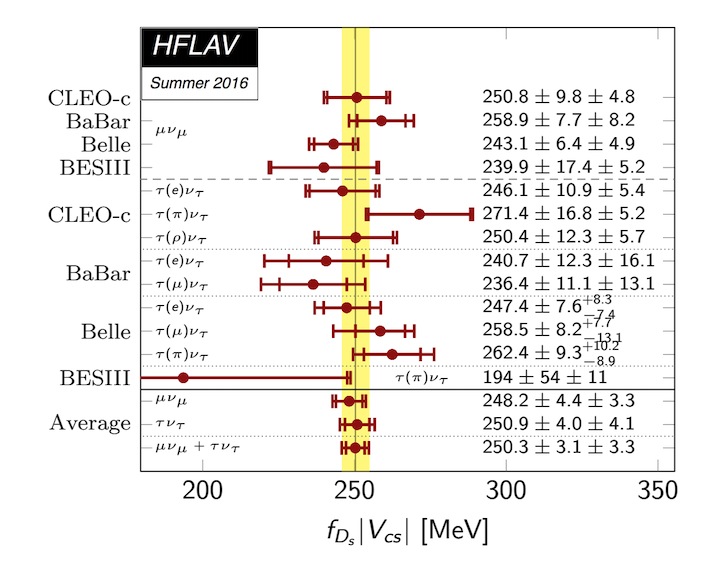
\includegraphics[width=0.45\textwidth]{vcs_meson_ds.png} \qquad
    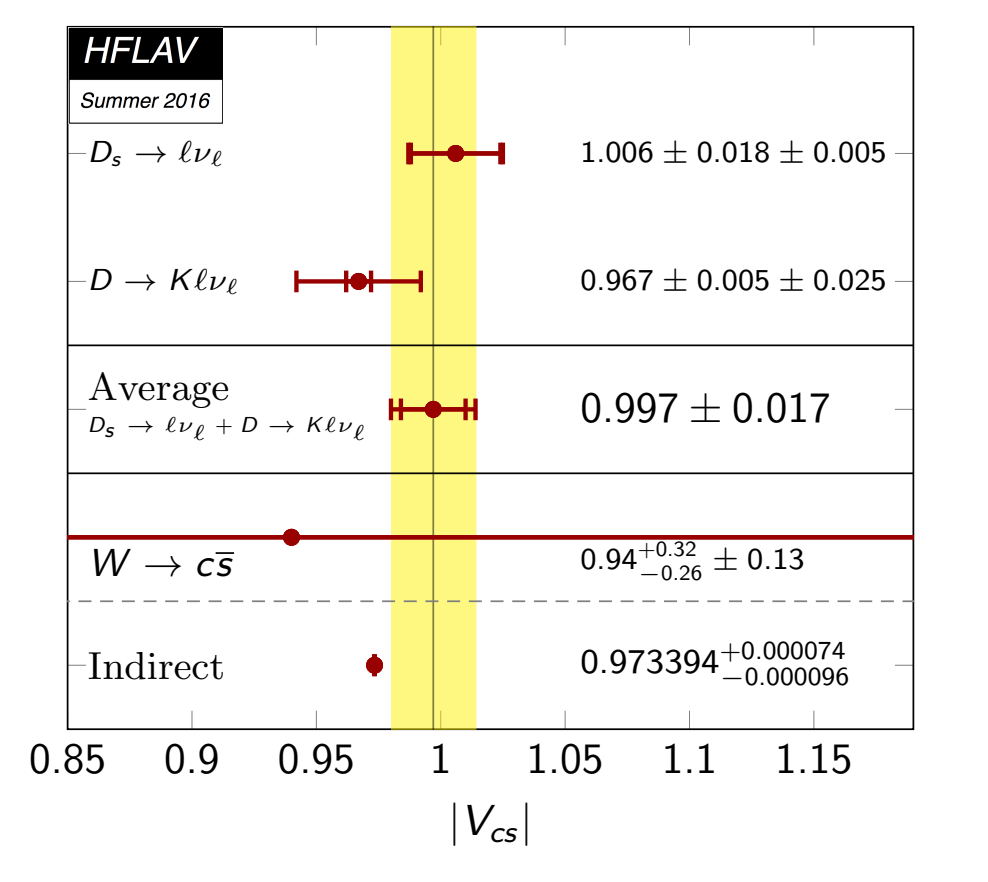
\includegraphics[width=0.6\textwidth]{chapters/RelatedWorks/sectionVcs/figures/vcs.png}
    \caption{The world average of $|V_{cs}|$ measurements. }
    \label{fig:relatedWorks:vcs:measurements}
\end{figure}




\subsection{Derive $V_{cs}$ from $B(W\to l \nu)$}


The coupling of W to lepton current is $g$ while to the quark current is $g|V_{ij}|$. 

\begin{equation}
    \feynmandiagram [inline=(d.base), small, horizontal=d to b] {
        a[particle=\(\nu_e\)] -- [fermion] b [dot] -- [fermion] c[particle=\(e^-\)],
        b -- [boson] d [particle=\(W^-\)],
    };
    = i g \gamma^{\mu} \qquad
    \feynmandiagram [inline=(d.base), small, horizontal=d to b] {
        a[particle=\(q_j\)] -- [fermion] b [dot] -- [fermion] c[particle=\(q_i\)],
        b -- [boson] d [particle=\(W^-\)],
    };
    = i g |V_{ij}|
\end{equation}

\noindent If we define the partial width of W to the lepton current $\Gamma_{W \to l \nu}$ as $\Gamma_l$, 

\begin{equation}
\Gamma_l \equiv \Gamma_{W \to l \nu} =  \frac{g^2 m_W}{48 \pi} .
\end{equation}


\noindent  At tree-level, the W decay width to the quark current is

\begin{equation}
\Gamma_{W \to q_i q_j}^{LO} = 3 |V_{ij}|^2 \frac{g^2 m_W}{48 \pi}  = 3 |V_{ij}|^2 \Gamma_l ,
\end{equation}

\noindent  where the factor 3 accounts for the three colors.

\begin{figure}
    \centering
    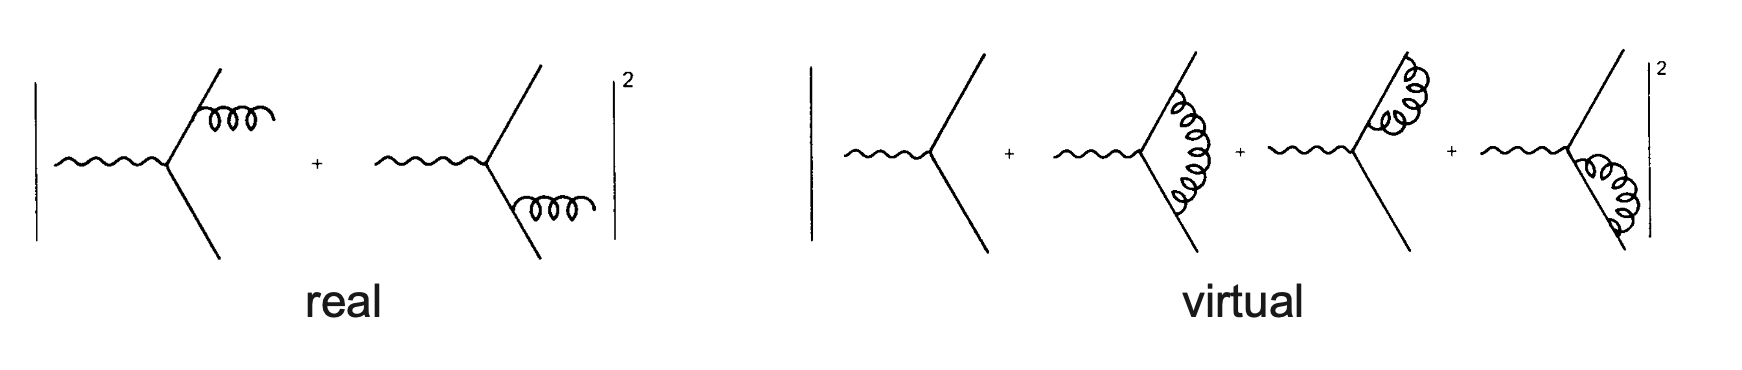
\includegraphics[width=0.8\textwidth]{chapters/RelatedWorks/sectionVcs/figures/realVirtual.png}
    \caption{ The real and virtual diagram of W decay considering the leading order QCD correction. }
    \label{fig:relatedWorks:vcs:realVirtual}
\end{figure}

\noindent However, at the NLO, QCD correction related to the quark current has to considered. More specifically, the real and virtual diagram, shown in Figure~\ref{fig:relatedWorks:vcs:realVirtual}, add extra contributions to the leading order width $\Gamma_{W \to q_i q_j}^{LO} $. The real diagram corresponds to the gluon final state radiation from the outcoming quarks. The virtual diagram corresponds to the interference between the tree level non-QCD process and the virtual gluon bubbles in the quark current and at the vertex. The calculation of the real and virtual contribution is usually expressed as a $k$ factor times the tree level rate  $\Gamma_{W \to q_i q_j}^{LO} $.
 
 \begin{align}
 	\Gamma^V_{W \to q_i q_j}  &= \Gamma_{W \to q_i q_j}^{LO} \times \frac{\alpha_s}{2\pi}\frac{4}{3} \bigg \{  -\ln^2\frac{m_g}{Q} -3 \ln\frac{m_g}{Q} + \frac{\pi^2}{3}-\frac{7}{2} \bigg\} \\
    \Gamma^R_{W \to q_i q_j}  &= \Gamma_{W \to q_i q_j}^{LO} \times \frac{\alpha_s}{2\pi}\frac{4}{3} \bigg \{  +\ln^2\frac{m_g}{Q} + 3 \ln\frac{m_g}{Q} - \frac{\pi^2}{3}+ 5 \bigg\}
 \end{align}
 
\noindent  where $Q$ is the energy of W boson and $m_g$ is the mass of the massless gluon, which makes both the real and virtual width diverge. But the divergences in the real and virtual rate when $\lim m_g \to 0$ exactly cancel each other, producing a fine total contributions to the tree level width. This QCD correction turns out to be a $k$ factor of $\frac{\alpha_s}{\pi}$ :

\begin{equation}
\begin{split}
    \Gamma_{W \to q_i q_j}^{NLO} =& \Gamma_{W \to q_i q_j}^{LO} + \Gamma^{V}_{W \to q_i q_j}  + \Gamma^{R}_{W \to q_i q_j}
            =   \Gamma_{W \to q_i q_j}^{LO} \big( 1+ \frac{\alpha_s(M_W)}{\pi}\big)
%             =&  \Gamma_l \bigg[ 1+ \frac{\alpha_s(M_W)}{\pi} \bigg]  \sum_{color} \sum_{ i,j } |V_{ij}|^2  \\
%             =&  \Gamma_l \bigg[ 1+ \frac{ \alpha_s(\mu_R) - \alpha^2_s(\mu_R) \frac{ \beta_0}{2\pi} \ln \frac{M_W}{\mu_R}}{\pi} \bigg] \sum_{color} \sum_{ i,j } |V_{ij}|^2  
\end{split} .
\end{equation}

\noindent The factor of QCD contributions has been calculated with higher order corrections upto 3NLO. The state-of-art result of this factor reads $k = 1+1.045 ( \frac{\alpha_s}{\pi} ) + 0.94  ( \frac{\alpha_s}{\pi} ) ^2 -15  ( \frac{\alpha_s}{\pi} ) ^3$. For calculation in this work, the NLO is good enough. By definition, the branching fraction of W satisfies the unitary constrain

\begin{equation}
    \sum_{ i,j } B_{W \to q_i q_j}^{NLO} + 3 B_l = 1
\end{equation}

\noindent use  $B_{W \to q_i q_j}^{NLO} = 3 (1+\frac{\alpha_s}{\pi}) |V_{ij}|^2 B_l $ and substitute $B_{W \to q_i q_j}^{NLO}$  with $B_l$ , one gets

\begin{equation}
    \sum_{ i,j } |V_{ij}|^2 = \frac{1}{ 1+ \alpha_s(M_W)/\pi } \, \frac{1-3B_l}{3B_l}
\end{equation}

\noindent where $\alpha_s(M_W) = \alpha_s(\mu_R) - \alpha^2_s(\mu_R) \frac{ \beta_0}{2\pi} \ln \frac{M_W}{\mu_R}$ and the renormalization scale is conventionally chosen as Z mass $\mu_R=M_Z$. The running couplings derived from the higher order of QCD renormalization group equation is discussed in the Section~\ref{sec:relatedWorks:qft:qcd}. The latest PDG value of $\alpha_s(m_Z)=0.1178\pm0.0010$. Using the leading order running of coupling, the $\alpha_s$ at W pole is
\begin{equation}
	\alpha_s(M_W) = 0.1199 \pm 0.0010
\end{equation}

\noindent  With $\sum_{ i,j } |V_{ij}|^2$ and the experimental value of other 5 better measured CKM elements \cite{pdg2020} in Table~\ref{tab:relatedWorks:vcs:ckm}, we can calculate the $V_{cs}$.



